\scanpage{128}
% archive sheet number: 127
% source lines 1--10
$B_{\handwritten{\alpha}}$ over the $A_{\handwritten{\alpha}}^{\handwritten{'}}$ which reduce to one another \ldots), \deleted{the $B$} moreover each $B_{\handwritten{\alpha}}$ being coflat over $A_{\handwritten{\alpha}}$. The preceding structure\inserted{\handwritten{$c$}}\handwritten{\begin{tikzpicture}[x=.35cm,y=.35cm,baseline=-.2ex]\draw (.15,-.5) .. controls (-.2,-.15) and (.4,.1) .. (.2,.4) .. controls (.1,.55) and (.1,.65) .. (.4,.7);\end{tikzpicture}} amounts to an isomorphism of \uline{b\deleted{i}}\deleted{m}\inserted{co}\uline{odules} over \deleted{$\unsure{B'|A'}\unsure{\otimes|\Omega}_{k}$} $A'$
\[
\begin{array}{l@{\qquad}l}(*)&B\otimes_{k'}B\handwritten{\unsure{\overset{\sim}{\Longleftarrow}|\xleftarrow{\sim}}}B\otimes_{k'}A'.\quad\deleted{\text{\unsure{From|By}}}\end{array}
\]
$\unsure{\rlap{\(\mathrm u\)}U|\mathbb U}$sing the augmentation of the factor $A'$, one deduces from this a homomorphism
\[
\begin{array}{l@{\qquad}l}(**)&B\otimes_{k'}B\handwritten{\longrightarrow}B\end{array}
\]
which will be a \uline{homomorphism of comodules} over $A'$ (NB use the multiplication of $A'$ to define the $A'$-comodule structure on the tensor product over $k$ of two such), i.e. one has a composition law on $B$ ``compatible with the $A'$-comodule structure''.
\margin{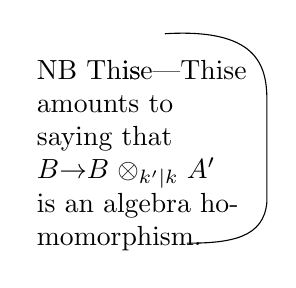
\begin{tikzpicture}[x=.35cm,y=.35cm,baseline=(n.base)]\node[anchor=north west,align=left,text width=2.7cm] (n) at (0,0) {NB \unsure{Th\rlap{i}i\rlap{s}s\deleted{e}|This\deleted{e}} amounts to saying that $B\handwritten{\to}B\otimes_{\unsure{k'|k}}A'$ is an algebra homomorphism.};\draw (5.0,.6) .. controls (8.3,.8) and (8.7,-.5) .. (8.7,-1.8)--(8.7,-5.5) .. controls (8.6,-6.8) and (7.4,-7.0) .. (5.8,-7.0);\end{tikzpicture}}
\margin{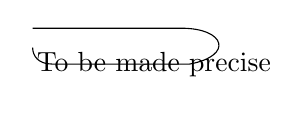
\begin{tikzpicture}[x=.35cm,y=.35cm,baseline=(n.base)]\node[anchor=north west,align=left] (n) at (0,0) {To be made precise};\draw (.2,.5)--(5.6,.5) .. controls (7.2,.5) and (7.5,-.5) .. (5.9,-.8)--(.9,-.8) .. controls (.4,-.8) and (.2,-.5) .. (.2,-.2);\end{tikzpicture}}\margin{\handwritten{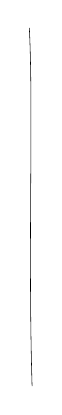
\begin{tikzpicture}[x=.35cm,y=.35cm,baseline=-.2ex]\draw[line width=.2pt] (0,0) .. controls (.15,-3) and (-.05,-8) .. (.1,-13);\end{tikzpicture}}}
\margin{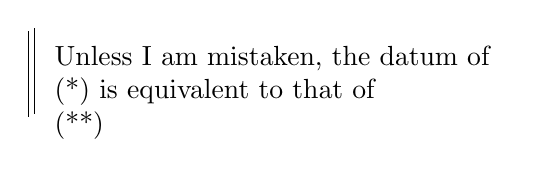
\begin{tikzpicture}[x=.35cm,y=.35cm,baseline=(n.base)]\node[anchor=north west,align=left,text width=5.6cm] (n) at (.6,0) {Unless I am mistaken, the datum of\\(*) \uline{is equivalent} \uline{to that of}\\(**)};\draw[line width=.5pt] (0,.2)--(0,-2.9);\draw[line width=.5pt] (.22,.3)--(.22,-2.8);\end{tikzpicture}}

% source lines 11--27
If $\handwritten{\Delta}$ on $U$ is unital i.e. $A$ is unital i.e. the $\otimes$ on $X$ \deleted{is admi \illegible{1}} admits a two-sided unit compatible with $F$, then the compatibility of $c$ with the units is expressed, unless I am mistaken, by the condition that the composition law (**) is unital.\deleted{(} Indeed, one must write that one has an isomorphism \deleted{$L\otimes_{\handwritten{U}}k$} $L\otimes_{U'}k'\handwritten{\simeq}k'$ satisfying certain conditions, now this amounts to giving oneself an\deleted{ element of} augmentation of $L$ satisfying a certain condition (namely \deleted{being compatible with}\inserted{being a two-sided unit for} the diagonal structure of $L$) or again an element of $B$ which is a two-sided unit.\inserted{This also implies that $B$ is \uline{faithfully} flat over $k'$.}\handwritten{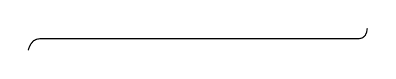
\begin{tikzpicture}[x=.35cm,y=.35cm,baseline=-.2ex]\draw (0,-.3) .. controls (.1,.05) and (.25,.12) .. (.45,.12)--(12.0,.12) .. controls (12.2,.12) and (12.3,.3) .. (12.3,.5);\end{tikzpicture}}\handwritten{\begin{tikzpicture}[x=.35cm,y=.35cm,baseline=-.2ex]\draw[line width=.5pt] (0,.05) .. controls (1,-.15) and (1.4,.3) .. (1.3,.7);\end{tikzpicture}} Similarly, if $\handwritten{\Delta}$ is associative, i.e.\inserted{if}\handwritten{
\begin{tikzpicture}[x=.35cm,y=.35cm,baseline=-.2ex]\draw (0,.5) .. controls (-.2,0) and (.1,-.4) .. (.4,-.2)--(1,-.2) .. controls (1.3,-.2) and (1.1,.2) .. (1.4,.35);\end{tikzpicture}} one has for $\otimes$ a d\deleted{t}atum of associativity $\handwritten{\phi}$ compatible with $F$, then $c$ is compatible with it if and only if $B$ is an associative algebra. \deleted{When the two conditions are verifi} Finally, when $\handwritten{\Delta}$ is commutative i.e. $C$ with $\handwritten{\psi}$ a symmetry datum, \ldots\ then $c$ is compatible with the latter, and the usual symmetry datum on $\unsure{\mathrm{P}\rlap{\(\mathrm r\)}\mathrm o\rlap{\(\mathrm r\)}\mathrm o\mathrm{jf}|\mathrm{Poojf}}(k')$ if and only if the composition law of $B$ is \deleted{asso} commutative. \handwritten{[}(But then, in terms of the affine monoid $\handwritten{\unsure{\rlap{\(G\)}H|H|G|\mathscr{H}|\mathscr{G}}}$ defined by $A$ over $k$, one sees that the structures of $B$ are expressed in terms of\inserted{\handwritten{$P:$}}\handwritten{\begin{tikzpicture}[x=.35cm,y=.35cm,baseline=-.2ex]\draw (0,-.3)--(.4,-.15)--(1.3,.9);\end{tikzpicture}} $\mathrm{Spec}\ B$ by saying that $\handwritten{{\rlap{\(G\)}H}_{k'}}$ acts on it on the right,\inserted{\handwritten{and $P$ is formally\textsuperscript{\handwritten{\begin{tikzpicture}[x=.35cm,y=.35cm,baseline=-.2ex]\draw[line width=.4pt] (.08,.35)--(.06,.1) .. controls (.05,.02) and (.09,-.02) .. (.13,.01);\end{tikzpicture}}} principal homogeneous}}\handwritten{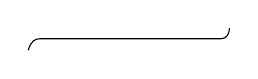
\begin{tikzpicture}[x=.35cm,y=.35cm,baseline=-.2ex]\draw (0,-.3) .. controls (.1,.05) and (.25,.12) .. (.45,.12)--(7.0,.12) .. controls (7.2,.12) and (7.3,.3) .. (7.3,.5);\end{tikzpicture}} and one sees moreover that after the chang\unsure{e}
\margin{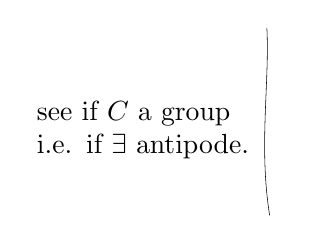
\begin{tikzpicture}[x=.35cm,y=.35cm,baseline=(n.base)]\node[anchor=north west,align=left,text width=3.0cm] (n) at (0,0) {\handwritten{see if $C$ a group i.e. if $\exists$ antipode.}};\draw[line width=.2pt] (8.7,2.3) .. controls (8.8,.3) and (8.4,-2.0) .. (8.8,-4.5);\end{tikzpicture}}
